\documentclass{beamer}

\usepackage{comment}
\usepackage{color}

\title{An Overview of the PFLOTRAN Input Deck}
\author{Glenn Hammond}
\date{\today}

\begin{document}

\frame{\titlepage}

\begin{frame}
%Freaking manual table of contents since beamer is stupid!!!!
\footnotesize
\begin{itemize}
\item[] {\color{blue}Syntax}
\item[] {\color{blue}Control Cards}
\begin{itemize}
\item[] SIMULATION
\end{itemize}
\item[] {\color{blue}Required Cards}
\begin{itemize}
\item[] GRID
\item[] REGION
\item[] MATERIAL\_PROPERTY
\item[] STRATA
\item[] TIME
\item[] INITIAL\_CONDITION
\end{itemize}
\item[] {\color{blue}Required Cards for Flow}
\begin{itemize}
\item[] FLOW\_CONDITION
\end{itemize}
\item[] {\color{blue}Required Cards for Reactive Transport}
\begin{itemize}
\item[] CHEMISTRY
\item[] TRANSPORT\_CONDITION
\item[] CONSTRAINT
\end{itemize}
\item[] {\color{blue}Optional Cards}
\begin{itemize}
\item[] OUTPUT
\item[] FLUID\_PROPERTY
\end{itemize}
\end{itemize}
\end{frame}

\section{Syntax}
\subsection{Syntax}

\begin{frame}[fragile,containsverbatim]\frametitle{Syntax}

The PFLOTRAN input deck is defined using keywords or cards that are associated with data.  The file is designed with modularity in mind and the cards need not be in any particular order.  Many cards open a section that provides additional cards and is terminated by an ``END'' or ``/''.  For example:

\begin{semiverbatim}
CARD1
  CARD2 value value
  CARD3
    CARD4 value
    CARD5 value
  /
END
\end{semiverbatim}

\end{frame}

\begin{frame}[fragile]\frametitle{Syntax: Commenting}
Several options exist for commenting out lines or sections of the input file:
\begin{itemize}
\item Individual lines may be commented out by placing a hash (\#) or exclamation point (!) at the beginning of line (i.e. before any text).
\item The SKIP/NOSKIP cards may be used to comment out a large number of lines.  SKIP/NOSKIP may be used in a nested manner.  
\item Comment characters (\# and !) may be used to place comments at the end of a line or to comment out the remainder of a line.
\end{itemize}

\end{frame}

\begin{frame}[containsverbatim]\frametitle{Syntax: Commenting Example}

\begin{semiverbatim}
CARD0
SKIP
CARD1
  ! comment on CARD2
  CARD2 value1 value2
  CARD3
  !  CARD4 value3 
    CARD5 value4 # comment explaining value3
  /
  CARD6 value5 ! comment explaining value5
#  CARD7 value6
  CARD7 value7
END
NOSKIP
CARD8
\end{semiverbatim}

\end{frame}


%-----------------------------------------------------------------------------
\section{Control Cards}

\subsection{SIMULATION}

\begin{frame}[fragile,containsverbatim]\frametitle{SIMULATION}

\begin{itemize}
\item[] \textbf{Purpose:} Defines 
\begin{itemize}
  \item Type of simulation
  \item Process models required
  \item Process model specific options
  \item Checkpoint/restart
\end{itemize}
\begin{comment}
\item[] \textbf{Example uses:}
\begin{itemize}
  \item 
\end{itemize}
\end{comment}
\item[] \textbf{Key sub-cards:}
\begin{itemize}
\item[] \verb|SIMULATION_TYPE|
\item[] \verb|  SUBSURFACE|
\item[] \verb|  HYDROGEOPHYSICS|
\item[] \verb|  GEOMECHANICS_SUBSURFACE|
\item[] \verb|  ...|
\item[] \verb|PROCESS_MODELS|
\item[] \verb|  SUBSURFACE_FLOW|
\item[] \verb|  SUBSURFACE_TRANSPORT|
\item[] \verb|  UFD_DECAY|
\item[] \verb|  ...|
\item[] \verb|CHECKPOINT|
\item[] \verb|RESTART|
\end{itemize}
\end{itemize}

\end{frame}

%-----------------------------------------------------------------------------
\begin{frame}[fragile]\frametitle{SIMULATION Example: Flow and Transport}

\begin{semiverbatim}
SIMULATION
  SIMULATION_TYPE SUBSURFACE
  PROCESS_MODELS
    SUBSURFACE_FLOW flow
      MODE RICHARDS
    /
    SUBSURFACE_TRANSPORT transport
      GLOBAL_IMPLICIT
    /
  /
END
\end{semiverbatim}

\end{frame}

%-----------------------------------------------------------------------------
\begin{frame}[fragile]\frametitle{SIMULATION Example: Multiphase Flow}

\begin{semiverbatim}
SIMULATION
  SIMULATION_TYPE SUBSURFACE
  PROCESS_MODELS
    SUBSURFACE_FLOW flow
      MODE GENERAL
      OPTIONS
        ANALYTICAL_JACOBIAN
        ARITHMETIC_GAS_DIFFUSIVE_DENSITY
      /
    /
  /
END
\end{semiverbatim}

\end{frame}

%-----------------------------------------------------------------------------
\begin{frame}[fragile]\frametitle{SIMULATION Example: With Checkpointing}
\begin{semiverbatim}
SIMULATION
  SIMULATION_TYPE SUBSURFACE
  PROCESS_MODELS
    SUBSURFACE_FLOW flow
      MODE TH
    /
  /
  CHECKPOINT
    PERIODIC TIMESTEP 10
    PERIODIC TIME y 100.
    TIMES y 137.
    FORMAT HDF5
  /
END
\end{semiverbatim}

\end{frame}


%-----------------------------------------------------------------------------
\section{Required Cards}

\subsection{GRID}

\begin{frame}[fragile,containsverbatim]\frametitle{GRID}

\begin{itemize}
\item[] \textbf{Purpose:} Defines the physically discretized domain
\item[] \textbf{Example uses:}
\begin{itemize}
  \item Type of discretization [structured, unstructured]
  \item Extent of domain
  \item Grid resolution
  \item Specifying direction of gravity vector
\end{itemize}
\item[] \textbf{Key sub-cards:}
\begin{itemize}
  \item[] \verb|TYPE|
  \item[] \verb|  STRUCTURED|
  \item[] \verb|  UNSTRUCTURED|
  \item[] \verb|  UNSTRUCTURED_EXPLICIT|
  \item[] \verb|ORIGIN|
  \item[] \verb|BOUNDS|
  \item[] \verb|NXYZ|
  \item[] \verb|DXYZ|
\end{itemize}
\end{itemize}

\end{frame}

%-----------------------------------------------------------------------------
\begin{frame}[fragile]\frametitle{GRID Example: Cartesian Grid with BOUNDS}

\begin{semiverbatim}
GRID
  TYPE STRUCTURED
  NXYZ 16 16 16
  BOUNDS
    0.d0 0.d0 0.d0
    16.d0 16.d0 16.d0
  /
END
\end{semiverbatim}

\end{frame}

%-----------------------------------------------------------------------------
\begin{frame}[fragile]\frametitle{GRID Example: Cartesian Grid with DXYZ}

\begin{semiverbatim}
GRID
  TYPE STRUCTURED
  ORIGIN 0.d0 0.d0 0.d0
  NXYZ 5 4 3
  DXYZ
    10. 11. 12. 13. 14.
    13. 12. 11. 10.
    15. 20. 25.
  /
END
\end{semiverbatim}

\end{frame}

%-----------------------------------------------------------------------------
\begin{frame}[fragile]\frametitle{GRID Example: Explicit Unstructured Grid}

\begin{semiverbatim}
GRID
  TYPE UNSTRUCTURED_EXPLICIT ./mixed.uge
END
\end{semiverbatim}
\textit{mixed.uge contents}
\begin{semiverbatim}
CELLS 15
1 4.0625 4.0625 4.0625 5.20833
2 4.375 4.375 3.125 2.60417
...
15 1.25 3.75 0.3125 2.60417
CONNECTIONS 24
1 2 4.16667 4.16667 3.3333 6.25
1 3 3.75 3.75 3.75 8.8388
...
14 15 0.41667 3.75 0.41667 2.2097
\end{semiverbatim}

\end{frame}

\subsection{REGION}

\begin{frame}[fragile,containsverbatim]\frametitle{REGION}

\begin{itemize}
\item[] \textbf{Purpose:} Defines a region of the physically discretized domain
\item[] \textbf{Example uses:}
\begin{itemize}
  \item Specify a 0-3D zone
  \item Specify an individual grid cell through i,j,k indices
  \item Specify a list of grid cells
\end{itemize}
\item[] \textbf{Key sub-cards:}
\begin{itemize}
  \item[] \verb|BLOCK|
  \item[] \verb|COORDINATE|
  \item[] \verb|COORDINATES|
  \item[] \verb|FACE|
  \item[] \verb|  EAST, WEST, SOUTH, NORTH, BOTTOM, TOP|
  \item[] \verb|FILE|
  \item[] \verb|CARTESIAN_BOUNDARY|
\end{itemize}
\end{itemize}

\end{frame}

%-----------------------------------------------------------------------------
\begin{frame}[fragile]\frametitle{REGION Example: Infinite}

\begin{semiverbatim}
REGION all
  COORDINATES
    -1.d20 -1.d20 -1.d20
    1.d20 1.d20 1.d20
  /
END
\end{semiverbatim}

\end{frame}

%-----------------------------------------------------------------------------
\begin{frame}[fragile]\frametitle{REGION Example: Plane}

\begin{semiverbatim}
REGION north
  FACE NORTH
  COORDINATES
    0.d0 46.d0 0.d0
    60.d0 46.d0 60.d0
  /
END
\end{semiverbatim}

\end{frame}

%-----------------------------------------------------------------------------
\begin{frame}[fragile]\frametitle{REGION Example: Point}

\begin{semiverbatim}
REGION center_of_13
  COORDINATE 1.25d0 2.91667 1.25d0
END
\end{semiverbatim}

\end{frame}

%-----------------------------------------------------------------------------
\begin{frame}[fragile]\frametitle{REGION Example: Line}

\begin{semiverbatim}
REGION well
  BLOCK 4 4 2 3 3 3
END
\end{semiverbatim}

\end{frame}

%-----------------------------------------------------------------------------
\begin{frame}[fragile]\frametitle{REGION Example: List of cell faces in file}

\begin{semiverbatim}
REGION west
  file west_of_12.ss
END
\end{semiverbatim}

\textit{west\_of\_12.ss contents}
\begin{semiverbatim}
1
Q 24 20 19 23
\end{semiverbatim}

\end{frame}



\subsection{MATERIAL\_PROPERTY}

\begin{frame}[fragile,containsverbatim]\frametitle{MATERIAL\_PROPERTY}

\begin{itemize}
\item[] \textbf{Purpose:} Define material properties for simulation.
\item[] \textbf{Example uses:}
\begin{itemize}
  \item Associate ID with material properties
  \item Specify porosity, permeability, rock/soil particle density
  \item Associate constitutive relations (e.g. saturation functions, relative permeability functions)
\end{itemize}
\item[] \textbf{Key sub-cards:}
\begin{itemize}
  \item[] \verb|ID|
  \item[] \verb|POROSITY|
  \item[] \verb|TORTUOSITY|
  \item[] \verb|PERMEABILITY|
  \item[] \verb|ROCK_DENSITY|
  \item[] \verb|SPECIFIC_HEAT|
  \item[] \verb|CHARACTERISTIC_CURVES|
  \item[] \verb|SOIL_COMPRESSIBILITY|
\end{itemize}
\end{itemize}

\end{frame}

%-----------------------------------------------------------------------------
\begin{frame}[fragile]\frametitle{MATERIAL\_PROPERTY Example: Solute Transport}

\begin{semiverbatim}
MATERIAL_PROPERTY soil
  ID 1
  POROSITY 0.25d0
  TORTUOSITY 1.d0
END
\end{semiverbatim}

\end{frame}

%-----------------------------------------------------------------------------
\begin{frame}[fragile]\frametitle{MATERIAL\_PROPERTY Example: Single Phase}

\begin{semiverbatim}
MATERIAL_PROPERTY soil1
  ID 1
  POROSITY 0.25d0
  TORTUOSITY 1.d0
  SOIL_COMPRESSIBILITY_FUNCTION LEIJNSE
  SOIL_COMPRESSIBILITY 1.d-7
  SOIL_REFERENCE_PRESSURE 1.d5
  PERMEABILITY
    PERM_ISO 1.d-12
  /
  CHARACTERISTIC_CURVES sf1
END
\end{semiverbatim}

\end{frame}

%-----------------------------------------------------------------------------
\begin{frame}[fragile]\frametitle{MATERIAL\_PROPERTY Example: MultiPhase}

\begin{semiverbatim}
MATERIAL_PROPERTY sand
  ID 1
  CHARACTERISTIC_CURVES cc1
  POROSITY 0.25
  TORTUOSITY 0.5
  ROCK_DENSITY 2650.d0 kg/m^3
  THERMAL_CONDUCTIVITY_DRY 0.6d0 W/m-C
  THERMAL_CONDUCTIVITY_WET 1.9d0 W/m-C
  HEAT_CAPACITY 830.d0 J/kg-C
  PERMEABILITY
    PERM_X 1.1d-12
    PERM_Y 1.d-12
    PERM_Z 1.d-12
  /
/
\end{semiverbatim}

\end{frame}

\subsection{STRATA}

\begin{frame}[fragile,containsverbatim]\frametitle{STRATA}

\begin{itemize}
\item[] \textbf{Purpose:} Ties material properties to regions of the physical domain
\item[] \textbf{Example uses:}
\begin{itemize}
  \item Define material IDs for grid cells
  \item Define transient material IDs
\end{itemize}
\item[] \textbf{Key sub-cards:}
\begin{itemize}
  \item[] \verb|REGION|
  \item[] \verb|MATERIAL|
  \item[] \verb|START_TIME|
  \item[] \verb|FINAL_TIME|
\end{itemize}
\end{itemize}

\end{frame}

%-----------------------------------------------------------------------------
\begin{frame}[fragile]\frametitle{STRATA Example: Simple}

\begin{semiverbatim}
STRATA
  REGION layer1
  MATERIAL soil1
END
\end{semiverbatim}

\end{frame}

%-----------------------------------------------------------------------------
\begin{frame}[fragile]\frametitle{STRATA Example: Transient}
\footnotesize
\begin{semiverbatim}
STRATA
  REGION rPCS
  MATERIAL PCS_T1
  START_TIME 0 y
  FINAL_TIME 100 y
END

STRATA
  REGION rPCS
  MATERIAL PCS_T2
  START_TIME 100 y
  FINAL_TIME 200 y
END
 
STRATA
  REGION rPCS
  MATERIAL PCS_T3
  START_TIME 200 y
  FINAL_TIME 10000 y
END
\end{semiverbatim}

\end{frame}

\subsection{TIME}

\begin{frame}[fragile,containsverbatim]\frametitle{TIME}

\begin{itemize}
\item[] \textbf{Purpose:} Defines temporal extent and discretization of simulation
\item[] \textbf{Example uses:}
\begin{itemize}
  \item Specify final time
  \item Specify time step size for a span of simulation
\end{itemize}
\item[] \textbf{Key sub-cards:}
\begin{itemize}
  \item[] \verb|FINAL_TIME|
  \item[] \verb|INITIAL_TIMESTEP_SIZE|
  \item[] \verb|MINIMUM_TIMESTEP_SIZE|
  \item[] \verb|MAXIMUM_TIMESTEP_SIZE|
\end{itemize}
\end{itemize}

\end{frame}

%-----------------------------------------------------------------------------
\begin{frame}[fragile]\frametitle{TIME Example: Mimimum Requirements}

\begin{semiverbatim}
TIME
  FINAL_TIME 10.d0 y
  INITIAL_TIMESTEP_SIZE 1.d0 h
  MAXIMUM_TIMESTEP_SIZE 5.d-2 y
END
\end{semiverbatim}

\end{frame}

%-----------------------------------------------------------------------------
\begin{frame}[fragile]\frametitle{TIME Example: Complex Time Stepping}

\begin{semiverbatim}
TIME
  FINAL_TIME 2000.d0 d
  INITIAL_TIMESTEP_SIZE 1.d0 d
  MAXIMUM_TIMESTEP_SIZE 100.d0 d AT 100.0 d
  MAXIMUM_TIMESTEP_SIZE 0.1d0 d AT 1300.0 d
  MAXIMUM_TIMESTEP_SIZE 0.02d0 d AT 1300.105d0 d
  MAXIMUM_TIMESTEP_SIZE 100.d0 d AT 1300.2d0 d
  MAXIMUM_TIMESTEP_SIZE 0.1d0 d AT 1400.0 d
  MAXIMUM_TIMESTEP_SIZE 0.02d0 d AT 1400.06d0 d
  MAXIMUM_TIMESTEP_SIZE 100.d0 d AT 1400.1d0 d
END
\end{semiverbatim}

\end{frame}

\subsection{INITIAL\_CONDITION}

\begin{frame}[fragile,containsverbatim]\frametitle{INITIAL\_CONDITION}

\begin{itemize}
\item[] \textbf{Purpose:} Ties a flow and/or transport condition state variables to a region of the physical domain as initial conditions.
\item[] \textbf{Example uses:}
\begin{itemize}
  \item Define initial pressure
  \item Define initial concentration
\end{itemize}
\item[] \textbf{Key sub-cards:}
\begin{itemize}
  \item[] \verb|FLOW_CONDITION|
  \item[] \verb|TRANSPORT_CONDITION|
  \item[] \verb|REGION|
\end{itemize}
\end{itemize}

\end{frame}

%-----------------------------------------------------------------------------
\begin{frame}[fragile]\frametitle{INITIAL\_CONDITION Example: Simple}

\begin{semiverbatim}
INITIAL_CONDITION
  FLOW_CONDITION initial
  REGION plume
END
\end{semiverbatim}

\end{frame}


%-----------------------------------------------------------------------------
\begin{frame}[fragile]\frametitle{INITIAL\_CONDITION Example: Flow and Transport}

\begin{semiverbatim}
INITIAL_CONDITION
  FLOW_CONDITION initial
  TRANSPORT_CONDITION initial
  REGION all
END
\end{semiverbatim}

\end{frame}


\section{Required Cards for Flow}
\subsection{FLOW\_CONDITION}

\begin{frame}[fragile,containsverbatim]\frametitle{FLOW\_CONDITION}

\begin{itemize}
\item[] \textbf{Purpose:} Defines parameters/conditions to be associated with flow boundary and initial conditions
\item[] \textbf{Example uses:}
\begin{itemize}
  \item Specify a constant pressures on cell faces
  \item Specify a transient fluxes through cell faces
  \item Define a hydrostatic column of water
\end{itemize}
\item[] \textbf{Key sub-cards:}
\begin{itemize}
  \item[] \verb|TYPE|
  \item[] \verb|  DIRICHLET|
  \item[] \verb|  NEUMANN|
  \item[] \verb|  RATE|
  \item[] \verb|DATUM|
  \item[] \verb|GRADIENT|
  \item[] \verb|PRESSURE|
  \item[] \verb|FLUX|
  \item[] \verb|RATE|
\end{itemize}
\end{itemize}

\end{frame}

%-----------------------------------------------------------------------------
\begin{frame}[fragile]\frametitle{FLOW\_CONDITION Example: Undulating River}

\begin{semiverbatim}
FLOW_CONDITION river
  TYPE
    PRESSURE HYDROSTATIC
  /
  INTERPOLATION LINEAR
  DATUM LIST
    TIME_UNITS d
    0.d0 0.d0 0.d0 34.d0
    10.d0 0.d0 0.d0 39.d0
    50.d0 0.d0 0.d0 33.d0
    100.d0 0.d0 0.d0 34.d0
  /
  PRESSURE 101325 ! Pa
END
\end{semiverbatim}

\end{frame}

%-----------------------------------------------------------------------------
\begin{frame}[fragile]\frametitle{FLOW\_CONDITION Example: Transient Rainfall}

\begin{semiverbatim}
FLOW_CONDITION recharge
  TYPE
    FLUX NEUMANN
  /
  FLUX LIST
    TIME_UNITS yr
    DATA_UNITS cm/yr
    0.d0 25.d0
    1.d0 23.d0
    2.d0 27.d0
    3.d0 22.d0
    4.d0 24.d0
    5.d0 29.d0
  /
END
\end{semiverbatim}

\end{frame}

%-----------------------------------------------------------------------------
\begin{frame}[fragile]\frametitle{FLOW\_CONDITION Example: Permeability-Weighted Injection Well}

\begin{semiverbatim}
FLOW_CONDITION injection_well
  TYPE
    RATE SCALED_VOLUMETRIC_RATE NEIGHBOR_PERM
  /
  RATE 1 m^3/hr
END
\end{semiverbatim}

\end{frame}


\section{Required Cards for Reactive Transport}
\subsection{CHEMISTRY}

\begin{frame}[fragile,containsverbatim]\frametitle{CHEMISTRY}

\begin{itemize}
\item[] \textbf{Purpose:} Define aqueous chemistry for problem
\item[] \textbf{Example uses:}
\begin{itemize}
  \item Conservative solute transport
  \item Multicomponet biogeochemical transport
\end{itemize}
\item[] \textbf{Key sub-cards:}
\begin{itemize}
  \item[] \verb|PRIMARY_SPECIES|
  \item[] \verb|SECONDARY_SPECIES|
  \item[] \verb|IMMOBILE_SPECIES|
  \item[] \verb|MINERALS|
  \item[] \verb|MINERAL_KINETICS|
  \item[] \verb|SORPTION|
  \item[] \verb|ACTIVITY_COEFFICIENTS|
  \item[] \verb|RADIOACTIVE_DECAY_REACTION|
  
\end{itemize}
\end{itemize}

\end{frame}

%-----------------------------------------------------------------------------
\begin{frame}[fragile]\frametitle{CHEMISTRY Example: Solute Transport}

\begin{semiverbatim}
CHEMISTRY
  PRIMARY_SPECIES
    Tracer
    Tracer2
  /
  OUTPUT
    TOTAL
    ALL
  /
END
\end{semiverbatim}

\end{frame}

%-----------------------------------------------------------------------------
\begin{frame}[fragile]\frametitle{CHEMISTRY Example: Carbonate Chemistry}

\tiny
\begin{semiverbatim}
CHEMISTRY
  PRIMARY_SPECIES
    H+
    HCO3-
    Ca++
  /
  SECONDARY_SPECIES
    OH-
    CO3--
    CO2(aq)
    CaCO3(aq)
    CaHCO3+
    CaOH+
  /
  GAS_SPECIES
    CO2(g)
  /
  MINERALS
    Calcite
  /
  MINERAL_KINETICS
    Calcite
      RATE_CONSTANT 1.d-6 mol/m^2-sec
    /
  /
  DATABASE ../../../database/hanford.dat
  LOG_FORMULATION
  ACTIVITY_COEFFICIENTS TIMESTEP
  OUTPUT
    PH
    TOTAL
    ALL
  /
END
\end{semiverbatim}

\end{frame}

\subsection{TRANSPORT\_CONDITION}

\begin{frame}[fragile,containsverbatim]\frametitle{TRANSPORT\_CONDITION}

\begin{itemize}
\item[] \textbf{Purpose:} Couples constraints with a type of condition for an initial or boundary condition
\item[] \textbf{Example uses:}
\begin{itemize}
  \item Specifying concentrations 
  \item Specifying types of conditions
\end{itemize}
\item[] \textbf{Key sub-cards:}
\begin{itemize}
  \item[] \verb|TYPE|
  \item[] \verb|  DIRICHLET|
  \item[] \verb|  ZERO_GRADIENT|
  \item[] \verb|  DIRICHLET_ZERO_GRADIENT|
  \item[] \verb|CONSTRAINT_LIST|
  \item[] \verb|TIME_UNITS|
\end{itemize}
\end{itemize}

\end{frame}

%-----------------------------------------------------------------------------
\begin{frame}[fragile]\frametitle{TRANSPORT\_CONDITION Example: Steady}

\begin{semiverbatim}
TRANSPORT_CONDITION source_concentration
  TYPE DIRICHLET
  CONSTRAINT_LIST
    0.d0 source_constraint
  /
END
\end{semiverbatim}

\end{frame}

%-----------------------------------------------------------------------------
\begin{frame}[fragile]\frametitle{TRANSPORT\_CONDITION Example: Transient}

\begin{semiverbatim}
TRANSPORT_CONDITION inlet_conc
  TYPE DIRICHLET_ZERO_GRADIENT
  TIME_UNITS y
  CONSTRAINT_LIST
    0.d0 initial_constraint
    1.d0 pulse_constraint
    2.d0 initial_constraint
  /
END
\end{semiverbatim}

\end{frame}

\subsection{CONSTRAINT}

\begin{frame}[fragile,containsverbatim]\frametitle{CONSTRAINT}

\begin{itemize}
\item[] \textbf{Purpose:} A snapshot of chemistry
\item[] \textbf{Example uses:}
\begin{itemize}
  \item Defining aqueous chemistry
  \item Defining mineralogy
\end{itemize}
\item[] \textbf{Key sub-cards:}
\begin{itemize}
  \item[] \verb|CONCENTRATIONS|
  \item[] \verb|SURFACE_COMPLEXES|
  \item[] \verb|IMMOBILE|
  \item[] \verb|MINERALS|
\end{itemize}
\end{itemize}

\end{frame}

%-----------------------------------------------------------------------------
\begin{frame}[fragile]\frametitle{CONSTRAINT Example: Solutes}

\begin{semiverbatim}
CONSTRAINT initial
  CONCENTRATIONS
    Tracer  1.d-10 T
    Tracer2 1.d-10 T
  /
END
\end{semiverbatim}

\end{frame}

%-----------------------------------------------------------------------------
\begin{frame}[fragile]\frametitle{CONSTRAINT Example: Carbonate Chemistry}

\begin{semiverbatim}
CONSTRAINT equilibrated
  CONCENTRATIONS
    H+     1.d-8      F
    HCO3-  1.d-3      G  CO2(g)
    Ca++   5.d-4      M  Calcite
  /
  MINERALS
    Calcite 1.d-5 1.d0 m^2/m^3
  /
END
\end{semiverbatim}

\end{frame}


%-----------------------------------------------------------------------------
\section{Optional Cards}
\documentclass{beamer}

\usepackage{comment}
\usepackage{color}
\usepackage{tabbing}

\title{Types of PFLOTRAN Boundary Conditions\\ Basic}
\author{Glenn Hammond}
\date{\today}

\begin{document}

\frame{\titlepage}

%-----------------------------------------------------------------------------
\section{Flow}
\subsection{Types of Flow Conditions}

\begin{frame}[fragile,containsverbatim]\frametitle{Types of Flow Conditions}

\vspace{0.1in}
\centering
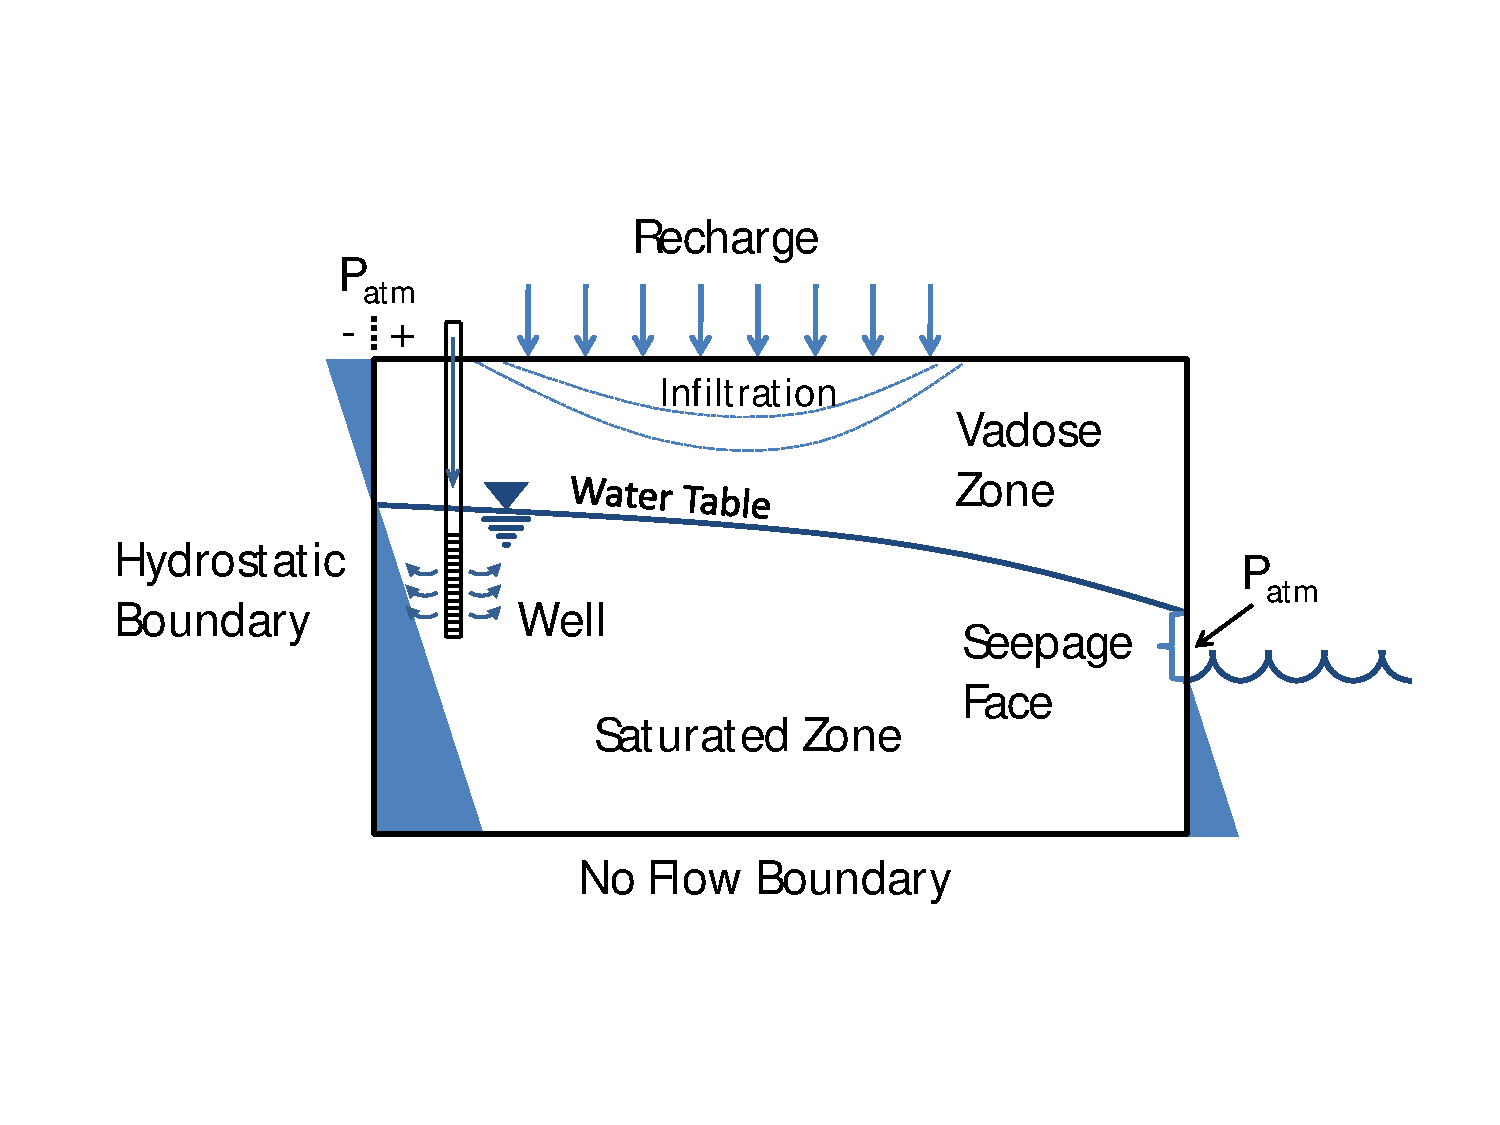
\includegraphics[width=0.9\linewidth]{./flow_bcs_with_well}
%\vspace{-0.5in}
\small 
\begin{tabbing}
\verb|DIRICHLET        |	\= Specified pressure across region\\
\verb|HYDROSTATIC|	      \> Hydrostatic pressure profile across region\\
\verb|SEEPAGE|	         	\> Hydrostatic with outflow only above water table\\
\verb|NEUMANN|			      \> Darcy flux across boundary [L/T]\\
\verb|MASS_RATE|	      	\> Mass injection/extraction rate [M/T]\\
\verb|VOLUMETRIC_RATE|	  \> Volumetric injection/extraction rate [L$^3$/T]\\
\end{tabbing}

\end{frame}


\section{Transport}
\subsection{Types of Transport Conditions}

\begin{frame}[fragile,containsverbatim]\frametitle{Types of Transport Conditions}

\vspace{0.1in}
\centering
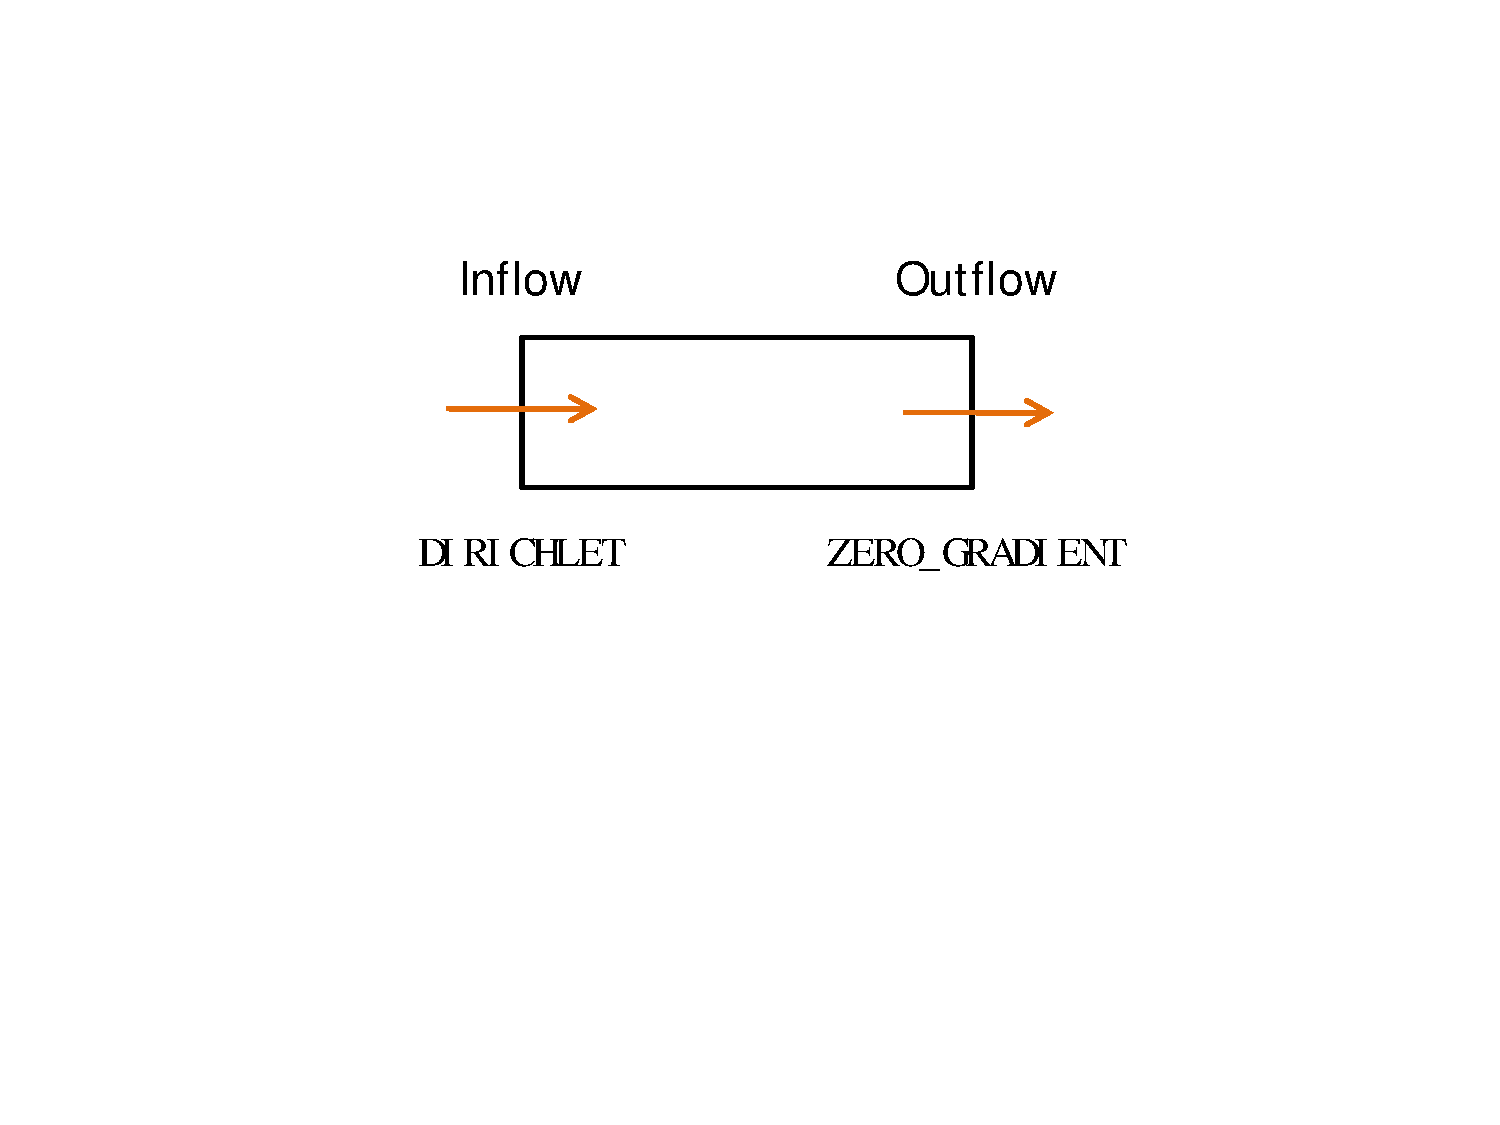
\includegraphics[width=0.5\linewidth]{./transport_bcs_unidirectional}
\vspace{0.1in}
%\hline
\vspace{0.1in}
\hspace{-6mm}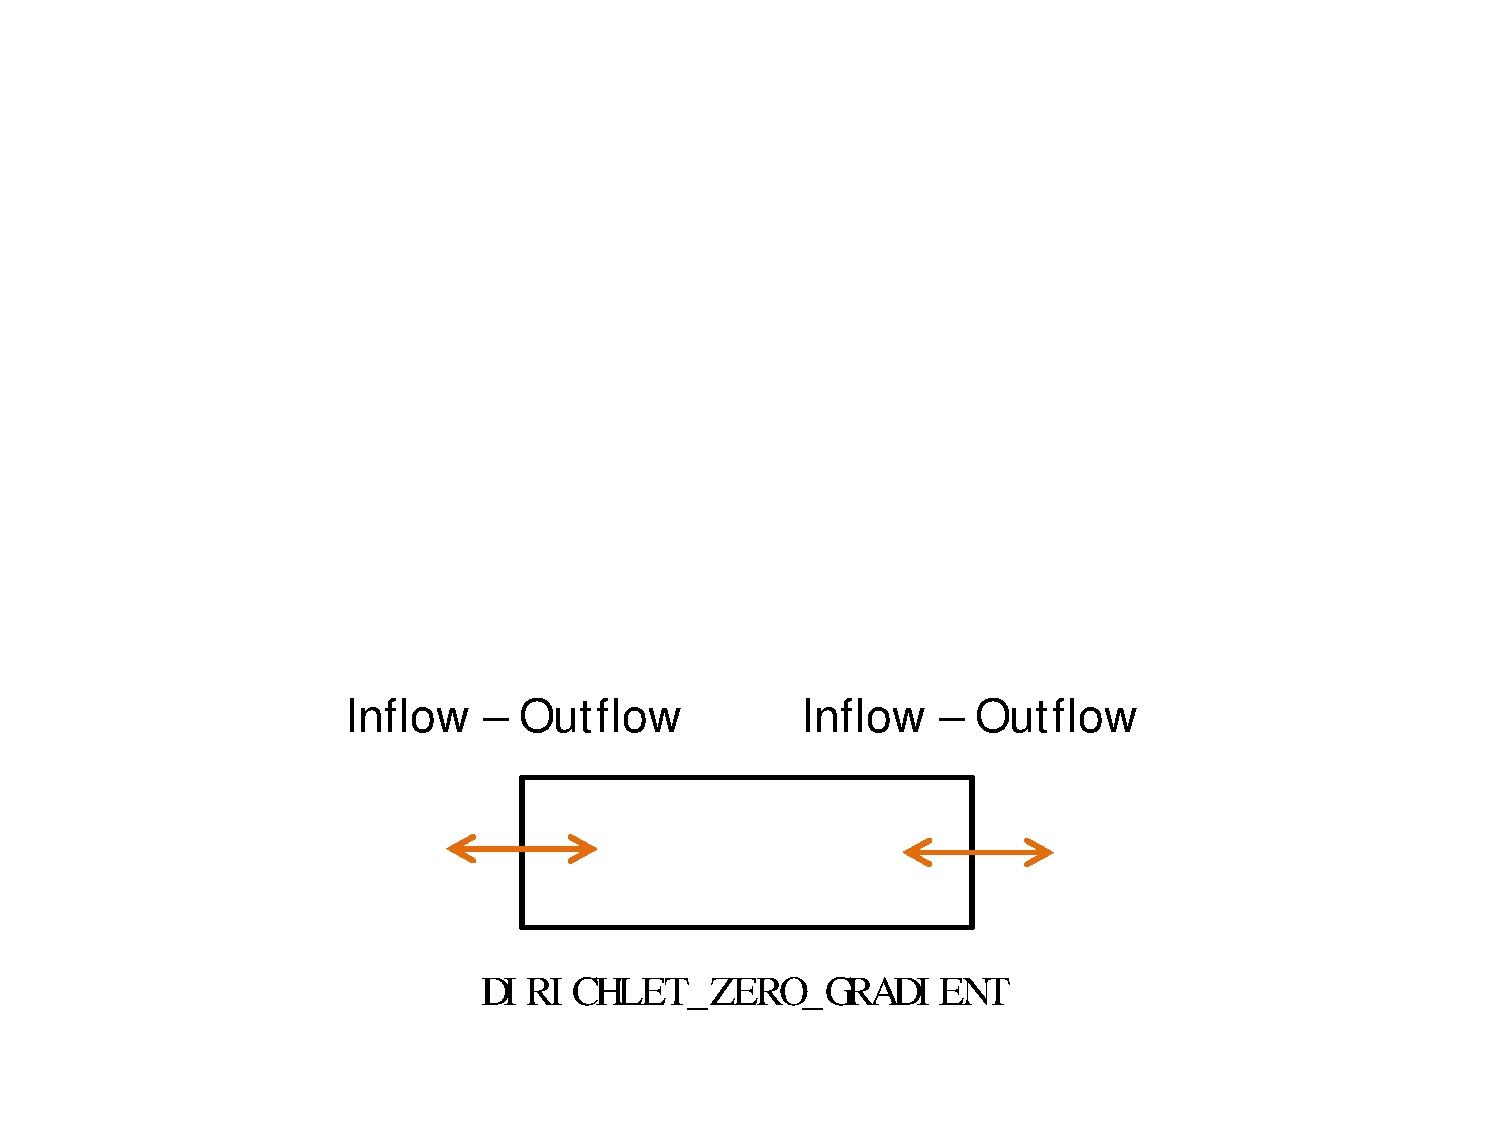
\includegraphics[width=0.58\linewidth]{./transport_bcs_bidirectional}

\begin{tabbing}
\verb|DIRICHLET                 |	\= Specified concentration\\
\verb|ZERO_GRADIENT|     	        \> Zero diffusive flux\\
\verb|DIRICHLET_ZERO_GRADIENT|		\> Hybrid for inflow - outflow
\end{tabbing}

\end{frame}




\end{document}
\subsection{OUTPUT}

\begin{frame}[fragile,containsverbatim]\frametitle{OUTPUT}

\begin{itemize}
\item[] \textbf{Purpose:} Defines file output for simulation.
\item[] \textbf{Example uses:}
\begin{itemize}
  \item Define times for plot file output
  \item Define times for observation point output
  \item Define output formatting
  \item Define output variables
\end{itemize}
\item[] \textbf{Key sub-cards:}
\begin{itemize}
  \item[] \verb|OBSERVATION_FILE|
  \item[] \verb|SNAPSHOT_FILE|
  \item[] \verb|MASS_BALANCE_FILE|
  \item[] \verb|VARIABLES|
  \item[] \verb|TIMES|
  \item[] \verb|FORMAT|
  \item[] \verb|  TECPLOT POINT|
  \item[] \verb|  HDF5|
\end{itemize}
\end{itemize}

\end{frame}

%-----------------------------------------------------------------------------
\begin{frame}[fragile]\frametitle{OUTPUT Example: Simple}

\begin{semiverbatim}
OUTPUT
  TIMES y 0.01 0.1 1.0
  FORMAT TECPLOT POINT
END
\end{semiverbatim}

\end{frame}

%-----------------------------------------------------------------------------
\begin{frame}[fragile]\frametitle{OUTPUT Example: Complex}

\begin{semiverbatim}
OUTPUT
  SNAPSHOT_FILE
    PERIODIC TIME 0.25 y BETWEEN 0. y AND 2. y
    PERIODIC TIME 1. y BETWEEN 0. y AND 10. y
    FORMAT TECPLOT BLOCK
    FORMAT HDF5
    PRINT_COLUMN_IDS
    VARIABLES
      LIQUID_PRESSURE
      LIQUID_SATURATION
    /
  /
  OBSERVATION_FILE
    PERIODIC TIMESTEP 1
  /
  VELOCITY_AT_CENTER
END
\end{semiverbatim}

\end{frame}

\subsection{FLUID\_PROPERTY}

\begin{frame}[fragile,containsverbatim]\frametitle{FLUID\_PROPERTY}

\begin{itemize}
\item[] \textbf{Purpose:} Define fluid properties
\item[] \textbf{Example uses:}
\begin{itemize}
  \item Set coefficient fo molecular diffusion
\end{itemize}
\item[] \textbf{Key sub-cards:}
\begin{itemize}
  \item[] \verb|DIFFUSION_COEFFICIENT|
\end{itemize}
\end{itemize}

\end{frame}

%-----------------------------------------------------------------------------
\begin{frame}[fragile]\frametitle{FLUID\_PROPERTY Example}

\begin{semiverbatim}
FLUID_PROPERTY 
  DIFFUSION_COEFFICIENT 1.d-9
END
\end{semiverbatim}

\end{frame}


\end{document}